\section{Programa p7.asm}

El código del programa se encuentra en un único archivo llamado \textbf{p7.asm}.
Este programa funciona mediante una aplicación de consola usando la api de 32
bits de Windows. Para la lectura del archivo se usan las funciones
CreateFile en modo lectura, GetFileSize y ReadFile el tamaño. Consiste en
leer un archivo de audio \textbf{.wav} y ``comprimirlo'' tomando solamente
muestras múltiplo de un valor m especificado por el usuario.

Se reutilizo gran parte del código de \cite{pract6} específicamente
en la apertura del archivo, el procedimiento de conversión numérica y
la lógica de escritura del archivo. La principal diferencia en esta
practica fue que el archivo posee un formato en especifico, por lo
cual requiere de una lógica que maneje conservar la estructura del
archivo y modificando algunos valores de cabecera ``ChunkSize'' y ``Chunk2Size''.


El programa se estructura de forma secuencial ejecutando los siguientes
pasos:

\begin{itemize}

\item{La primera parte es la apertura de los archivos de escritura y lectura, esta
    fue explicada previamente en \cite{pract6}.}

\item{Solicita la la entrada de un entero m por parte del usuario y
    mediante el uso de una rutina se convierte de cadena de caracteres a un entero.}

\item{Se lee en la cabecera del archivo original, el \textbf{BlockAlign} el
    cual indica la cantidad de bytes que constituye una muestra.}

\item{Se ajusta los valores de cabecera, del nuevo archivo y se escribe
    en el archivo final.}

\item{Se ejecuta un ciclo, el cual toma muestras del archivo anterior,
    moviéndose en saltos de m y las escribe directamente en el nuevo archivo.}

\item{Finalmente se guarda el archivo final, y se termina la ejecución del programa.}

\end{itemize}


Antes de la escritura del archivo se calcula cuantas iteraciones hacen
falta para escribir el nuevo archivo y esto se obtiene mediante
la lectura del tamaño del bloque de data, y este se divide por el factor
ingreso por el usuario, luego este valor llamado \textbf{new\_data\_size}
se divide nuevamente entre el \textbf{BlockAlign} (Cantidad de canales $\times$
cantidad de bytes por muestra) y de esta forma se obtiene la cantidad
de iteraciones necesarias para la escritura del archivo.

Al momento de escribir en el archivo se utiliza un contador y debido
a que los datos están escritos de forma secuencial se utiliza la formula
$direccion\_inicial = base + m\times n \times frame\_size$
para obtener la dirección inicial a partir de la cual comenzara la escritura
del frame\_size bytes en el nuevo archivo. Cabe resaltar que frame\_size
es \textbf{BlockAlign}.

\begin{figure}[!ht]
\centering
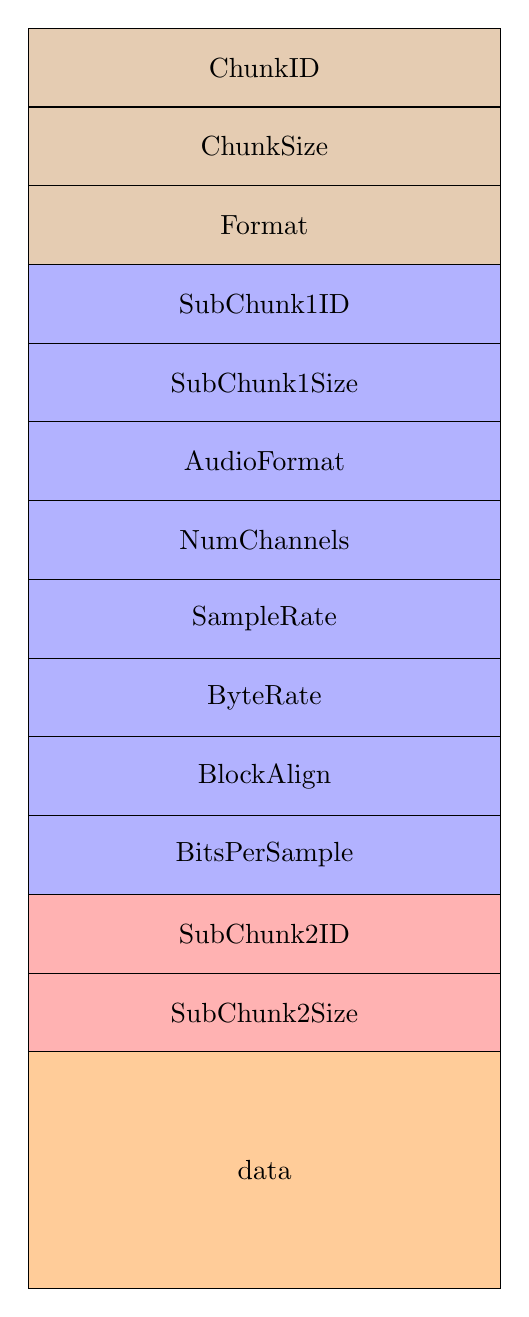
\begin{tikzpicture}

\foreach \name \y in {ChunkID/1, ChunkSize/2, Format/3}{
    \filldraw[fill=brown!40!white] (0,-\y) rectangle node {\name} (6,-\y+1);
}

\foreach  \name  \y in {SubChunk1ID/4, SubChunk1Size/5, AudioFormat/6, NumChannels/7, SampleRate/8, ByteRate/9, BlockAlign/10, BitsPerSample/11}{
    \filldraw[fill=blue!30!white] (0,-\y) rectangle node {\name} (6,-\y+1);
}

\foreach \name \y in {SubChunk2ID/12, SubChunk2Size/13}{
    \filldraw[fill=red!30!white] (0,-\y) rectangle node {\name} (6,-\y+1);
}
\filldraw[fill=orange!40!white] (0,-16) rectangle node {data} (6,-13);

\end{tikzpicture}
\caption{Estructura de un archivo .wav}
\end{figure}

\section*{Codigo del programa}

\lstinputlisting[language={[x86masm]Assembler}]{practica7/consola/p7.asm}

\section*{Funcionamiento del programa}

\begin{figure}[H]
  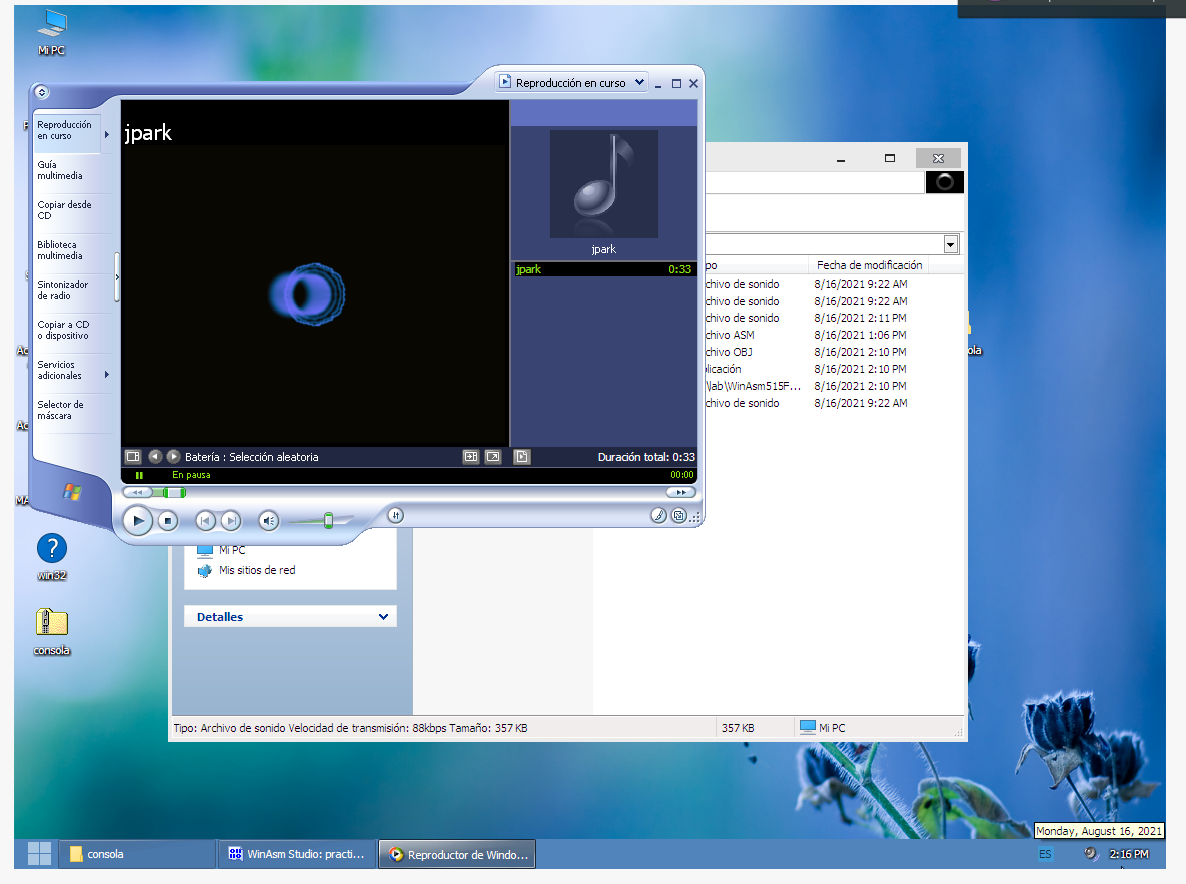
\includegraphics[width=\linewidth]{practica7/img/fig1}
    \caption{Archivo original}
\end{figure}

\begin{figure}[H]
  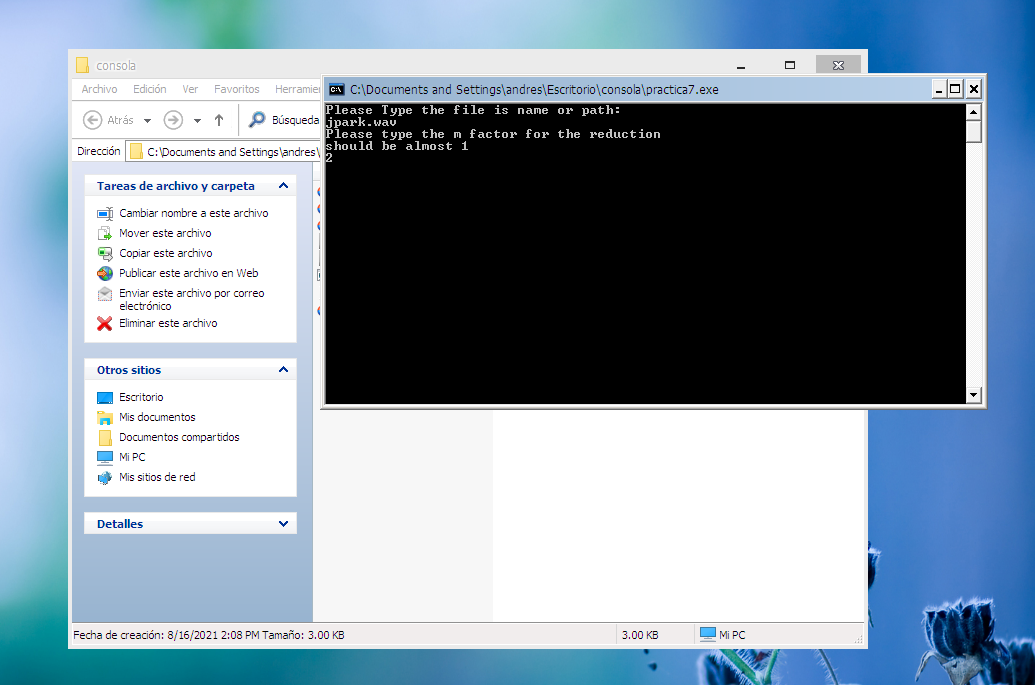
\includegraphics[width=\linewidth]{practica7/img/fig2}
    \caption{Ejecucion del programa}
\end{figure}

\begin{figure}[H]
  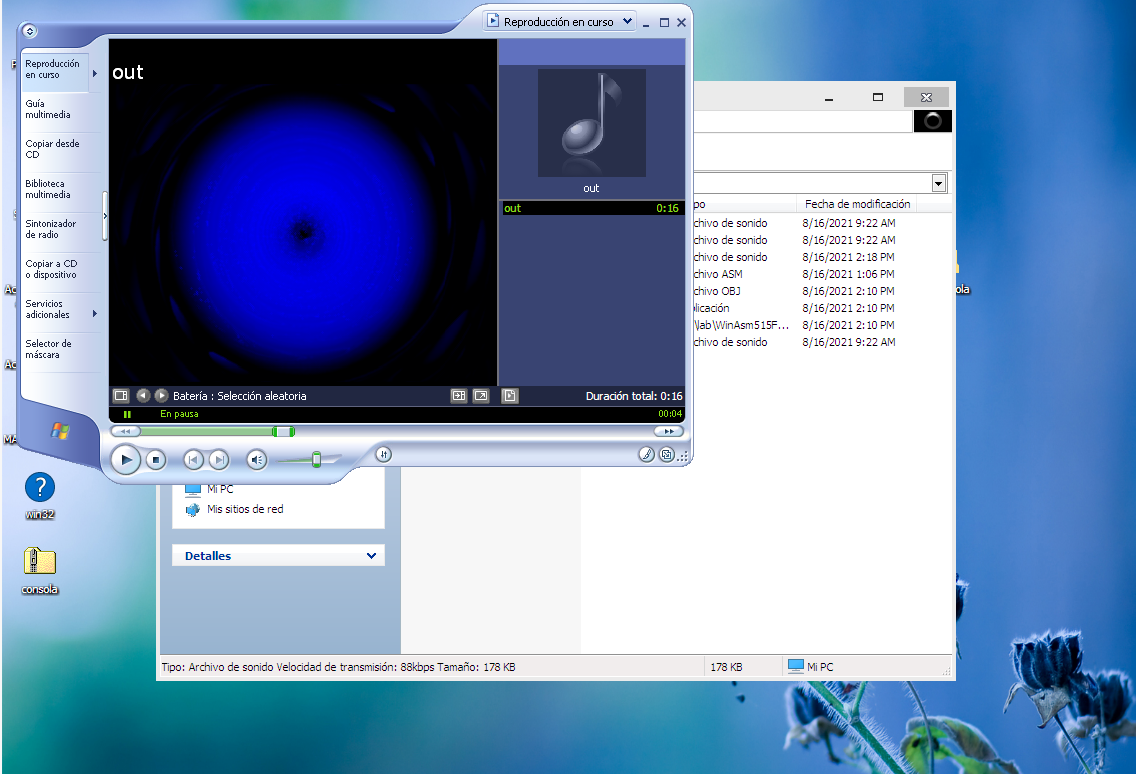
\includegraphics[width=\linewidth]{practica7/img/fig3}
    \caption{Archivo resultante}
\end{figure}
